\documentclass[journal,letterpaper]{IEEEtran}
\usepackage[utf8]{inputenc}
\usepackage[spanish]{babel}
\usepackage{amsmath}
\usepackage{graphicx}
\usepackage{booktabs}
\usepackage{hyperref}
\usepackage{microtype}
\usepackage{array}
\usepackage{multirow}
\graphicspath{{../../figures/}}

\begin{document}

\title{Reporte de Sprint 4: Integración del MVP, Validación Backtest, Explicabilidad SHAP y Storytelling de Negocio}

\author{Marcelo de la Quintana,
        Gaston Nina,
        y~Gerick Toro\\
        \textit{Módulo de Implementación de Soluciones de Inteligencia Artificial}\\
        \textit{Maestría en Inteligencia Artificial y Ciencia de Datos}}

\markboth{INFORME TÉCNICO - SPRINT 4, JUNIO 2026}%
{Sprint 4: MVP, Backtest y Demo Day}

\maketitle

\begin{abstract}
Este informe documenta el Sprint 4 del proyecto de identificación de clientes premium sobre Olist, cuyo objetivo fue transformar el modelo final del Sprint 3 en un MVP defendible para Demo Day, integrando un pipeline reproducible de scoring sobre una ventana de backtest, un dashboard en Streamlit, una API mínima, explicabilidad local y global, y una narrativa de impacto de negocio. El pipeline reutilizado genera \texttt{backtest\_features\_selected.parquet} alineado al esquema esperado por \texttt{modelo\_final.pkl}. Sobre el backtest de agosto de 2018 se obtuvo un ROC-AUC de \textbf{0.9876}, Gini de \textbf{0.9751}, Precision de \textbf{43.80\%}, Recall de \textbf{56.11\%} y F1-Score de \textbf{49.20\%}. Sin embargo, se argumenta que este desempeño no debe interpretarse de forma aislada como evidencia absoluta de generalización superior, ya que la etiqueta premium se define por gasto acumulado y el backtest presenta una población mucho más desbalanceada y estructuralmente más fácil que la validación de Sprint 3. A nivel de negocio, el modelo permite pasar de una campaña masiva con ROI estimado de \textbf{-89.57\%} a una campaña focalizada con ROI de \textbf{+250.40\%}, reduciendo el costo comercial en BRL \textbf{1,417,365.00}. La explicabilidad se reforzó con contribuciones locales nativas de LightGBM y un SHAP Summary Plot tipo beeswarm, mientras que la capa de gobernanza quedó documentada en términos de sesgo logístico, señales de pago y supervisión humana.
\end{abstract}

\begin{IEEEkeywords}
Streamlit, FastAPI, Docker, Backtest Temporal, SHAP, LightGBM, Clasificación Supervisada, Clientes Premium, Olist, ROI, Gobernanza de Modelos.
\end{IEEEkeywords}

\section{Introducción}
\IEEEPARstart{E}{l} Sprint 3 cerró con un modelo LightGBM tuneado serializado como \texttt{modelo\_final.pkl}, seleccionado por maximizar la discriminación global sobre el split temporal de desarrollo y validación (\texttt{last\_purchase} $<$ / $\geq$ 2018-07-01), alcanzando ROC-AUC$_{val}=0.8081$ y Gini$_{val}=0.6162$. El objetivo del \textbf{Sprint 4} fue convertir ese artefacto analítico en una demostración funcional y defendible para negocio, preservando reproducibilidad, explicabilidad y trazabilidad.

El sprint se organizó en cuatro bloques:
\begin{enumerate}
    \item Reutilización del pipeline para generar un dataset de scoring en \texttt{backtest}.
    \item Construcción del MVP en Streamlit y empaquetado reproducible en Docker.
    \item Validación analítica sobre backtest con métricas técnicas, explicabilidad y simulación financiera.
    \item Consolidación de narrativa ejecutiva, gobernanza y checklist de Demo Day.
\end{enumerate}

La pregunta central del Sprint 4 ya no es ``¿qué modelo rinde mejor?'', sino \textit{¿podemos demostrar que el modelo final es integrable, explicable y útil para una decisión comercial realista?}

\subsection{Angulo correcto de defensa}
Para exposición académica y ejecutiva conviene fijar una distinción explícita: \textbf{Sprint 3} es la validación metodológica principal del clasificador, mientras que \textbf{Sprint 4} es la validación de producto mínimo viable. Por ello, el resultado más importante del sprint no es ``mejorar'' artificialmente el AUC, sino demostrar cinco capacidades concretas:
\begin{enumerate}
    \item scoring reproducible sobre una ventana de backtest;
    \item integración funcional en dashboard y API;
    \item explicabilidad local y global con SHAP;
    \item traducción del score a impacto económico mediante ROI;
    \item documentación de riesgos, gobernanza y límites metodológicos.
\end{enumerate}

\section{Arquitectura del Sprint 4}
\subsection{Flujo técnico}
El flujo implementado sigue la secuencia:
\[
\texttt{backtest} \rightarrow \texttt{master\_table\_backtest}
\]
\[
\rightarrow \texttt{backtest\_features\_rfm} \rightarrow \texttt{backtest\_features\_selected}
\rightarrow \texttt{modelo\_final.pkl}
\]

\begin{figure}[h]
  \centering
  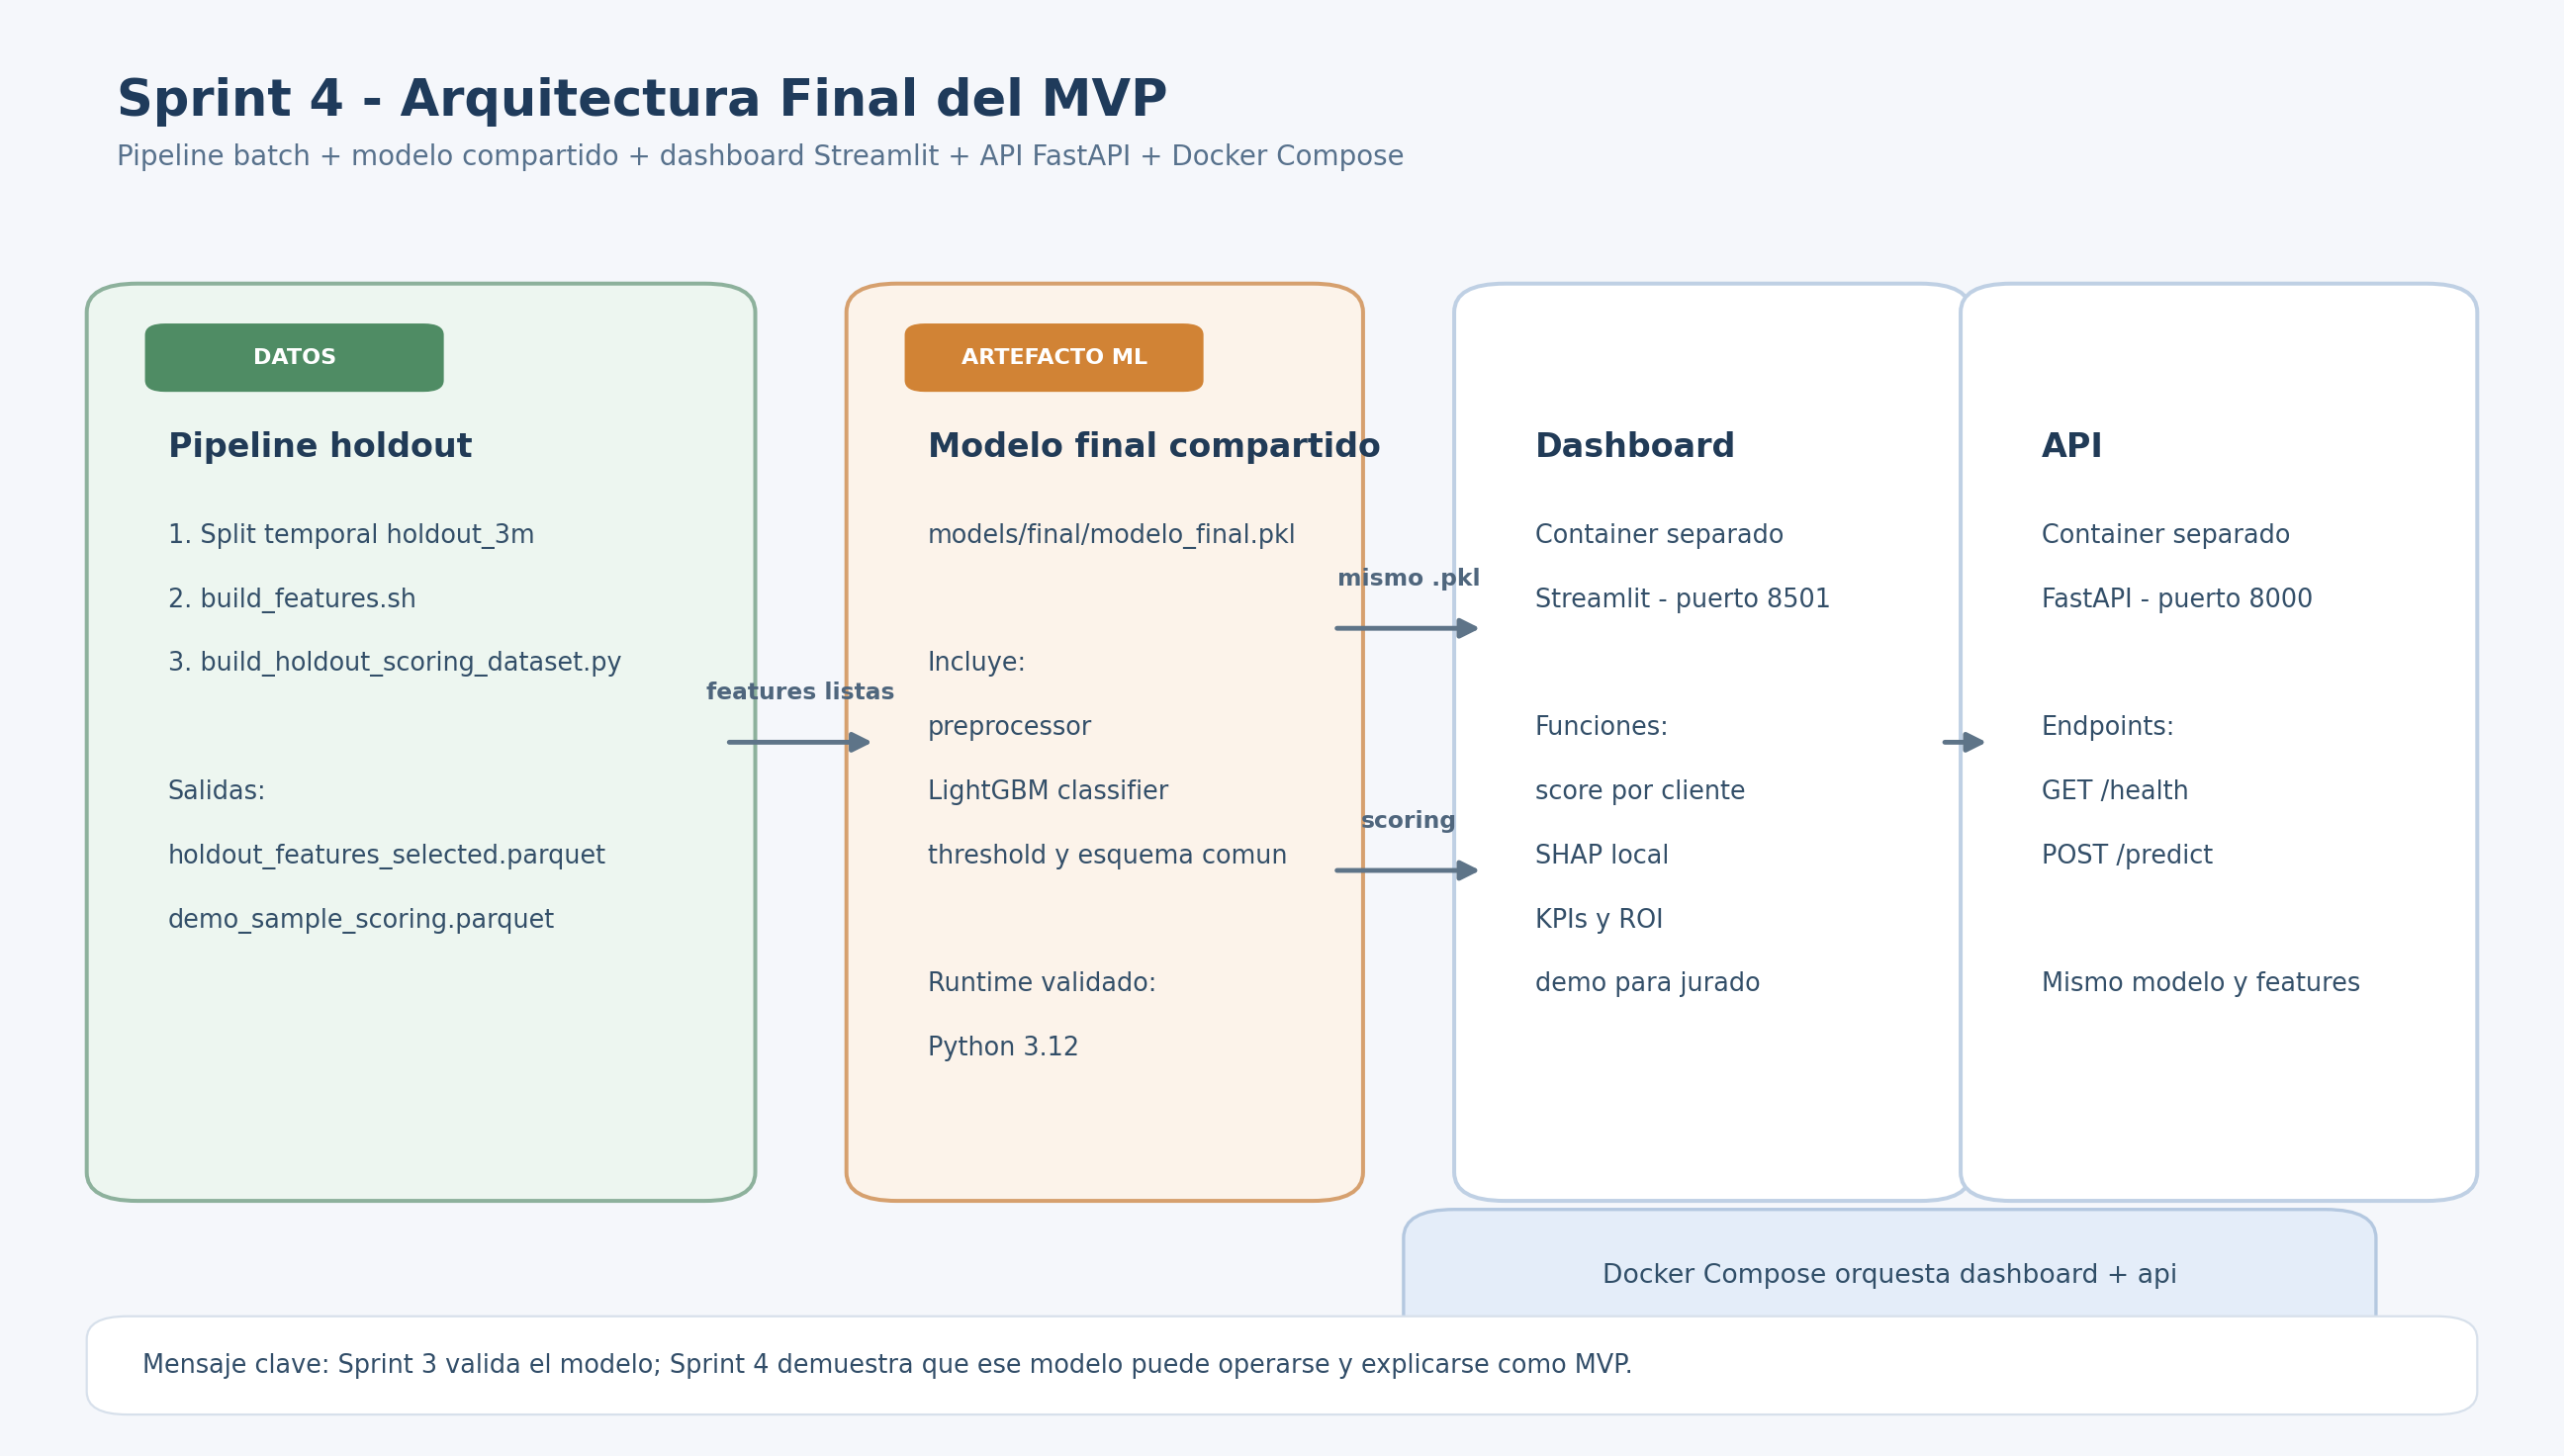
\includegraphics[width=\columnwidth]{sprint_04_mvp_architecture.png}
  \caption{Arquitectura final del MVP de Sprint 4. El pipeline prepara el dataset de scoring, mientras dashboard y API consumen el mismo artefacto del modelo dentro de contenedores separados.}
  \label{fig:mvp_architecture}
\end{figure}

Los entregables principales del sprint son:
\begin{itemize}
    \item \texttt{backtest\_features\_selected.parquet} y \texttt{demo\_sample\_scoring.parquet} en \texttt{data/processed/}.
    \item \texttt{app.py} del dashboard en \texttt{app/dashboard/}.
    \item \texttt{main.py} de la API en \texttt{app/api/}.
    \item Figuras principales del sprint en \texttt{reports/figures/}, incluyendo ROI y SHAP beeswarm.
\end{itemize}

\subsection{Compatibilidad operativa}
Tras regenerar el artefacto \texttt{modelo\_final.pkl} en un entorno actualizado, los contenedores del dashboard y la API se fijaron en Python 3.12. La validación realizada en Sprint 4 comprobó que el modelo se carga correctamente dentro de ambos contenedores Docker y mantiene compatibilidad operativa con el MVP.

\section{Validación Backtest}
\subsection{Definición del escenario backtest}
Aunque el split técnico histórico del proyecto conservó una partición \texttt{holdout\_3m} entre agosto y octubre de 2018, la distribución real de órdenes mostró que septiembre y octubre están prácticamente vacíos. Para evitar una evaluación final apoyada en una cola truncada, Sprint 4 formaliza como backtest la ventana completa de \textbf{agosto de 2018} (\texttt{backtest}) y aplica el mismo umbral de negocio persistido en desarrollo: un cliente es premium si su gasto acumulado en la ventana es mayor o igual al umbral fijo de BRL \textbf{197.01} (P80 del conjunto de desarrollo).

\begin{table}[h]
\centering
\caption{Resumen del Backtest Sprint 4}
\label{tab:backtest_summary}
\begin{tabular}{lr}
\toprule
Métrica & Valor \\
\midrule
Clientes evaluados & 96,096 \\
Clientes premium reales & 1,253 \\
Tasa premium real & 1.30\% \\
Clientes predichos como premium & 1,605 \\
Tasa premium predicha & 1.67\% \\
Umbral de clasificación & 0.55 \\
\bottomrule
\end{tabular}
\end{table}

\subsection{Métricas técnicas}
\begin{table}[h]
\centering
\caption{Métricas Técnicas sobre Backtest}
\label{tab:backtest_metrics}
\begin{tabular}{lr}
\toprule
Métrica & Valor \\
\midrule
ROC-AUC & 0.9876 \\
Gini & 0.9751 \\
Precision & 43.80\% \\
Recall & 56.11\% \\
F1-Score & 49.20\% \\
\bottomrule
\end{tabular}
\end{table}

\subsection{Interpretación crítica del ROC-AUC alto}
Aunque el ROC-AUC de \textbf{0.9876} es notablemente superior al ROC-AUC de validación del Sprint 3 (\textbf{0.8081}), esta diferencia no debe interpretarse automáticamente como una mejora masiva de generalización del modelo. Tampoco es evidencia directa de sobreajuste clásico, ya que el overfitting se manifiesta cuando el rendimiento en datos no vistos cae respecto al desarrollo, no cuando aumenta.

La explicación más plausible combina dos factores metodológicos:
\begin{enumerate}
    \item \textbf{La tarea en backtest es más fácil.} La población evaluada contiene una gran masa de clientes sin actividad o con actividad mínima en la ventana, mientras que el segmento premium exige al menos gasto suficiente para superar el umbral fijo. Esta separación estructural facilita la discriminación.
    \item \textbf{La etiqueta premium está muy acoplada a señales transaccionales.} Aunque se excluyeron variables de leakage directo como \texttt{total\_spent} y \texttt{avg\_ticket}, se conservaron proxies fuertes del comportamiento de gasto, como \texttt{delivered\_orders}, \texttt{total\_items}, \texttt{max\_payment\_installments} y \texttt{top\_category\_is\_high\_value}. Por ello, el modelo no memoriza el target, pero sí resuelve una tarea muy cercana al criterio de negocio que define la etiqueta.
\end{enumerate}

\subsection{Nota sobre el holdout historico de 3 meses}
El split \texttt{holdout\_3m} se mantiene en el repositorio por compatibilidad y trazabilidad del trabajo previo, pero no se usa ya como escenario oficial de evaluación final del Sprint 4. La razón es que septiembre y octubre de 2018 solo aportan 20 órdenes combinadas, por lo que no constituyen una ventana seria para juzgar desempeño. En consecuencia:
\begin{itemize}
    \item no interpretamos septiembre y octubre como evidencia de tendencia comercial;
    \item no usamos esa cola para sostener métricas finales del modelo;
    \item tratamos agosto de 2018 como backtest oficial y dejamos el holdout de tres meses como antecedente del recorte temporal.
\end{itemize}

En consecuencia, para defensa académica se recomienda presentar este AUC como \textbf{evidencia de fuerte separabilidad del escenario backtest}, no como prueba única de superioridad absoluta del modelo. La comparación metodológicamente correcta del modelo sigue siendo la validación temporal del Sprint 3.

\section{Explicabilidad}
\subsection{SHAP local y global}
La demo incorpora explicabilidad local por cliente mediante \texttt{pred\_contrib=True} de LightGBM sobre el espacio transformado por el \texttt{ColumnTransformer}. Adicionalmente, se generó un SHAP Summary Plot tipo beeswarm sobre una muestra del backtest.

\begin{figure}[h]
  \centering
  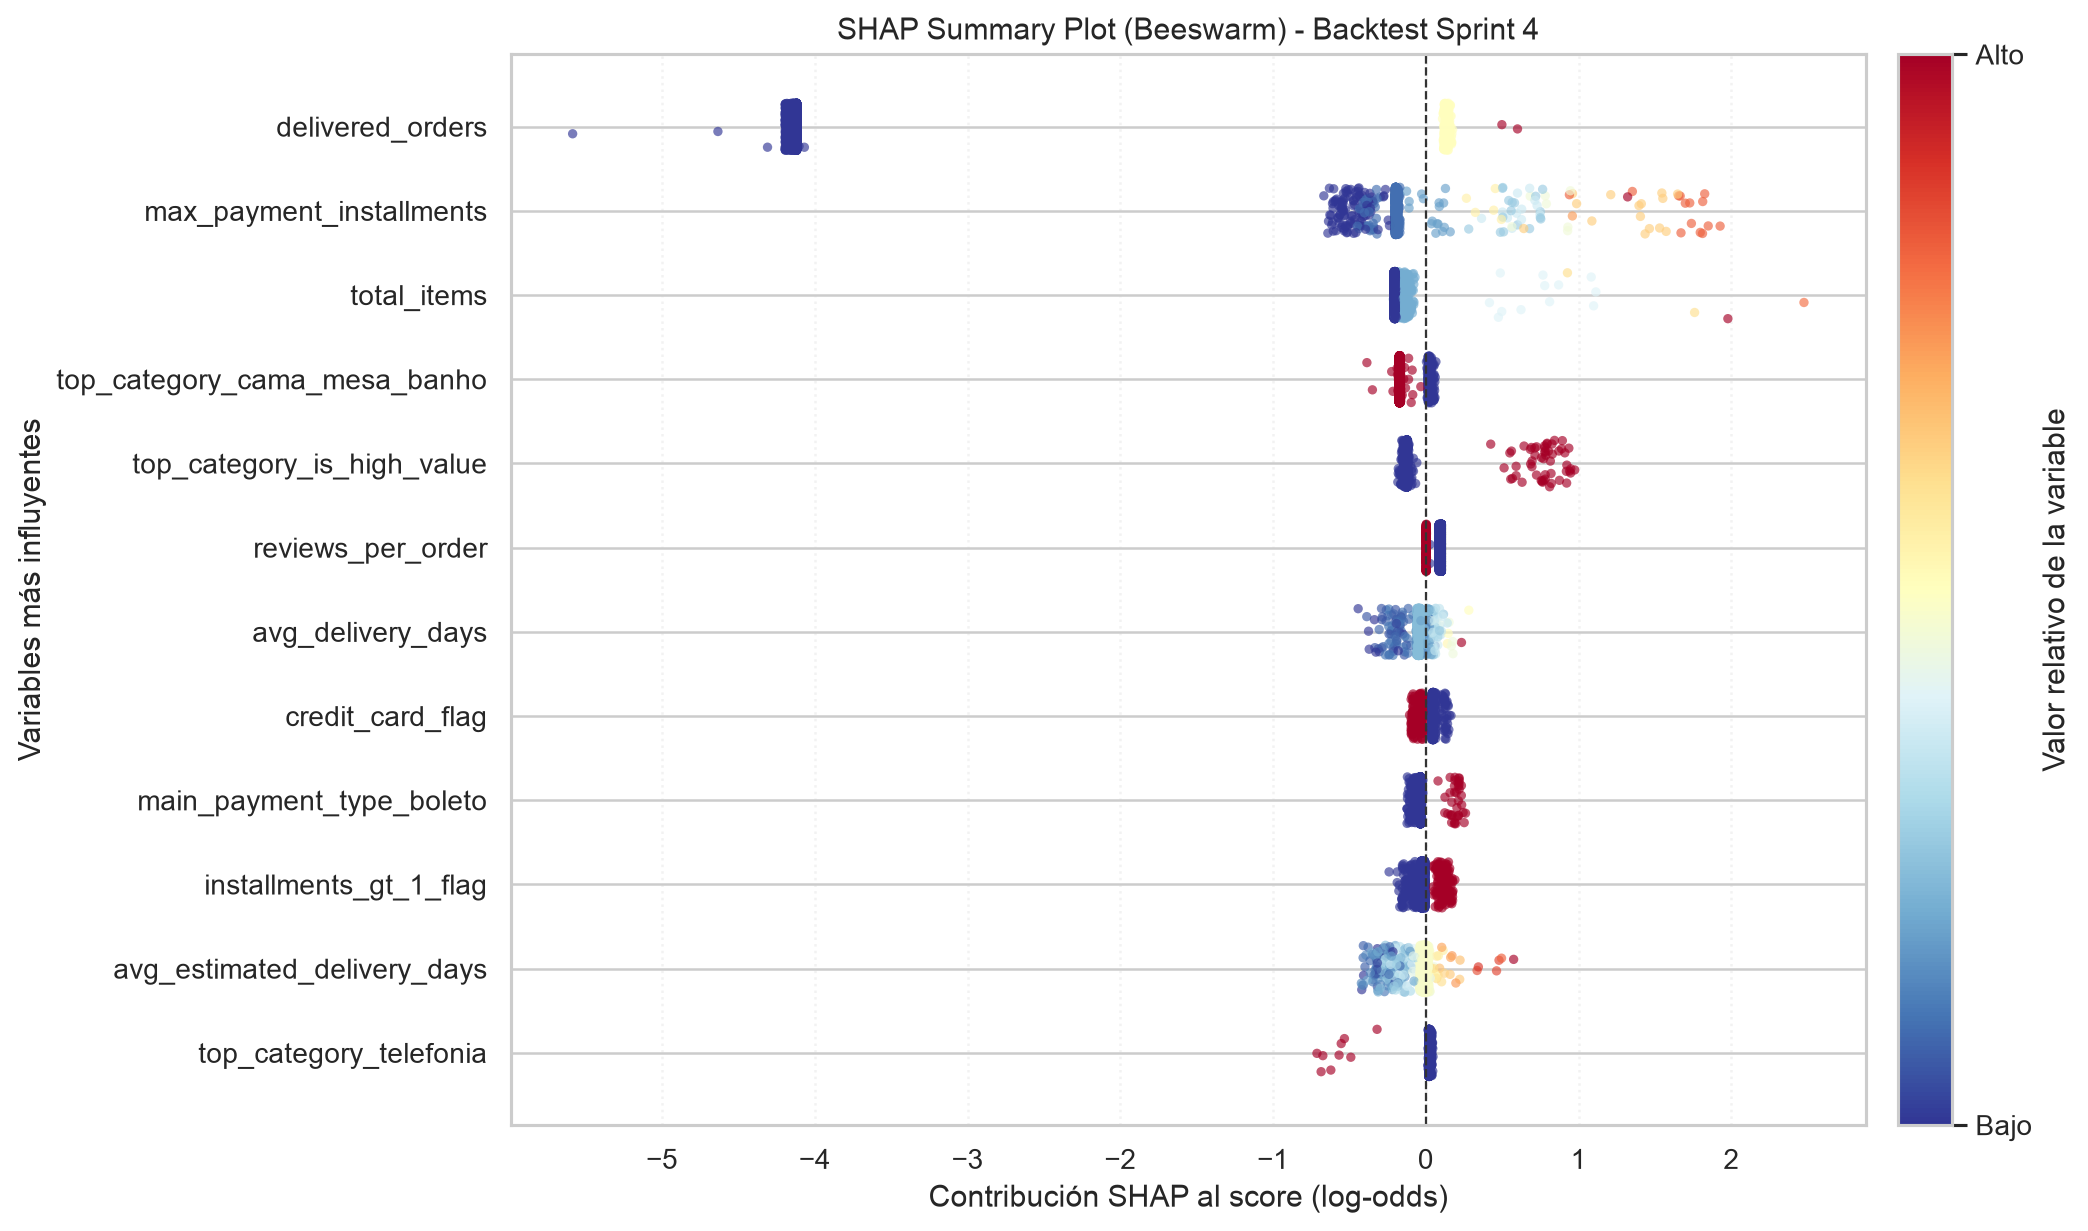
\includegraphics[width=\columnwidth]{sprint_04_shap_beeswarm.png}
  \caption{SHAP Summary Plot (beeswarm) sobre una muestra de 3,000 clientes del backtest. Las variables más influyentes son predominantemente transaccionales y de valor comercial.}
  \label{fig:shap_beeswarm}
\end{figure}

Las variables líderes del SHAP global son coherentes con la lógica del caso:
\begin{itemize}
    \item \texttt{delivered\_orders}
    \item \texttt{max\_payment\_installments}
    \item \texttt{total\_items}
    \item \texttt{top\_category\_is\_high\_value}
\end{itemize}

Esto refuerza la interpretación de que el modelo identifica intensidad transaccional, participación en categorías de alto valor y comportamiento de pago como señales dominantes del segmento premium.

\section{Impacto de Negocio}
\subsection{Simulación financiera}
Se compararon dos estrategias:
\begin{enumerate}
    \item \textbf{Campaña masiva}: contactar a toda la base.
    \item \textbf{Campaña focalizada}: contactar solo a clientes con probabilidad $\geq 0.55$.
\end{enumerate}

\begin{table}[h]
\centering
\caption{Comparativa de Estrategias Comerciales}
\label{tab:roi}
\resizebox{\columnwidth}{!}{%
\begin{tabular}{lrr}
\toprule
Métrica & Masiva & Modelo \\
\midrule
Clientes contactados & 96,096 & 1,605 \\
Costo de campaña & BRL 1,441,440.00 & BRL 24,075.00 \\
Ingreso por conversiones & BRL 150,360.00 & BRL 84,360.00 \\
Utilidad neta & BRL -1,291,080.00 & BRL 60,285.00 \\
ROI & -89.57\% & +250.40\% \\
\bottomrule
\end{tabular}%
}
\end{table}

\subsection{Lift y capacidad de priorización del ranking}
Además del umbral operativo, el docente solicitó validar la capacidad del score como ranking comercial. Para ello, ordenamos el backtest por probabilidad predicha descendente y lo dividimos en \textbf{10 deciles del mismo tamaño}. En cada decil medimos cuántos clientes premium reales aparecen, cuántos se acumulan y cuál es el \textit{lift} respecto a una selección aleatoria.

Esta lectura es especialmente valiosa para negocio porque responde una pregunta distinta a la de Precision/Recall: \textit{si solo priorizamos el 10\%, 20\% o 30\% de la base con mayor score, qué proporción del segmento premium logramos capturar?}

\begin{table}[h]
\centering
\caption{Tabla de Deciles Lift/Gain sobre Backtest}
\label{tab:lift_gain_backtest}
\resizebox{\columnwidth}{!}{%
\begin{tabular}{rrrrrrrr}
\toprule
Decil & Casos & Premium & \% premium decil & Premium acum. & Gain acum. (\%) & Lift & Lift acum. \\
\midrule
1 & 9,609 & 1,253 & 13.04 & 1,253 & 100.00 & 10.00 & 10.00 \\
2 & 9,610 & 0 & 0.00 & 1,253 & 100.00 & 0.00 & 5.00 \\
3 & 9,609 & 0 & 0.00 & 1,253 & 100.00 & 0.00 & 3.33 \\
4 & 9,610 & 0 & 0.00 & 1,253 & 100.00 & 0.00 & 2.50 \\
5 & 9,610 & 0 & 0.00 & 1,253 & 100.00 & 0.00 & 2.00 \\
6 & 9,609 & 0 & 0.00 & 1,253 & 100.00 & 0.00 & 1.67 \\
7 & 9,610 & 0 & 0.00 & 1,253 & 100.00 & 0.00 & 1.43 \\
8 & 9,609 & 0 & 0.00 & 1,253 & 100.00 & 0.00 & 1.25 \\
9 & 9,610 & 0 & 0.00 & 1,253 & 100.00 & 0.00 & 1.11 \\
10 & 9,610 & 0 & 0.00 & 1,253 & 100.00 & 0.00 & 1.00 \\
\bottomrule
\end{tabular}%
}
\end{table}

Los resultados muestran una concentración extrema del valor al inicio del ranking: el \textbf{primer decil} ya captura \textbf{100\%} de todos los premium reales del backtest y opera con un \textbf{lift de 10.00x}. Sin embargo, esto \textbf{no} significa que ese primer decil sea 100\% premium. En realidad, la tasa premium dentro del decil 1 es de \textbf{13.04\%}, frente a una tasa base total de apenas \textbf{1.30\%}. Es decir, el ranking multiplica por diez la densidad esperada de premium en el tramo más alto del score. A partir del segundo decil ya no aparecen nuevos premium reales. Esta evidencia es consistente con el ROC-AUC extraordinariamente alto del backtest y refuerza que el score no solo clasifica bien, sino que \textbf{ordena de manera muy agresiva la base para una campaña priorizada}. Al mismo tiempo, esta forma tan abrupta del ranking también confirma que agosto de 2018 es un escenario \textbf{mucho más fácil y separable} que la validación metodológica de Sprint 3.

\begin{figure}[h]
  \centering
  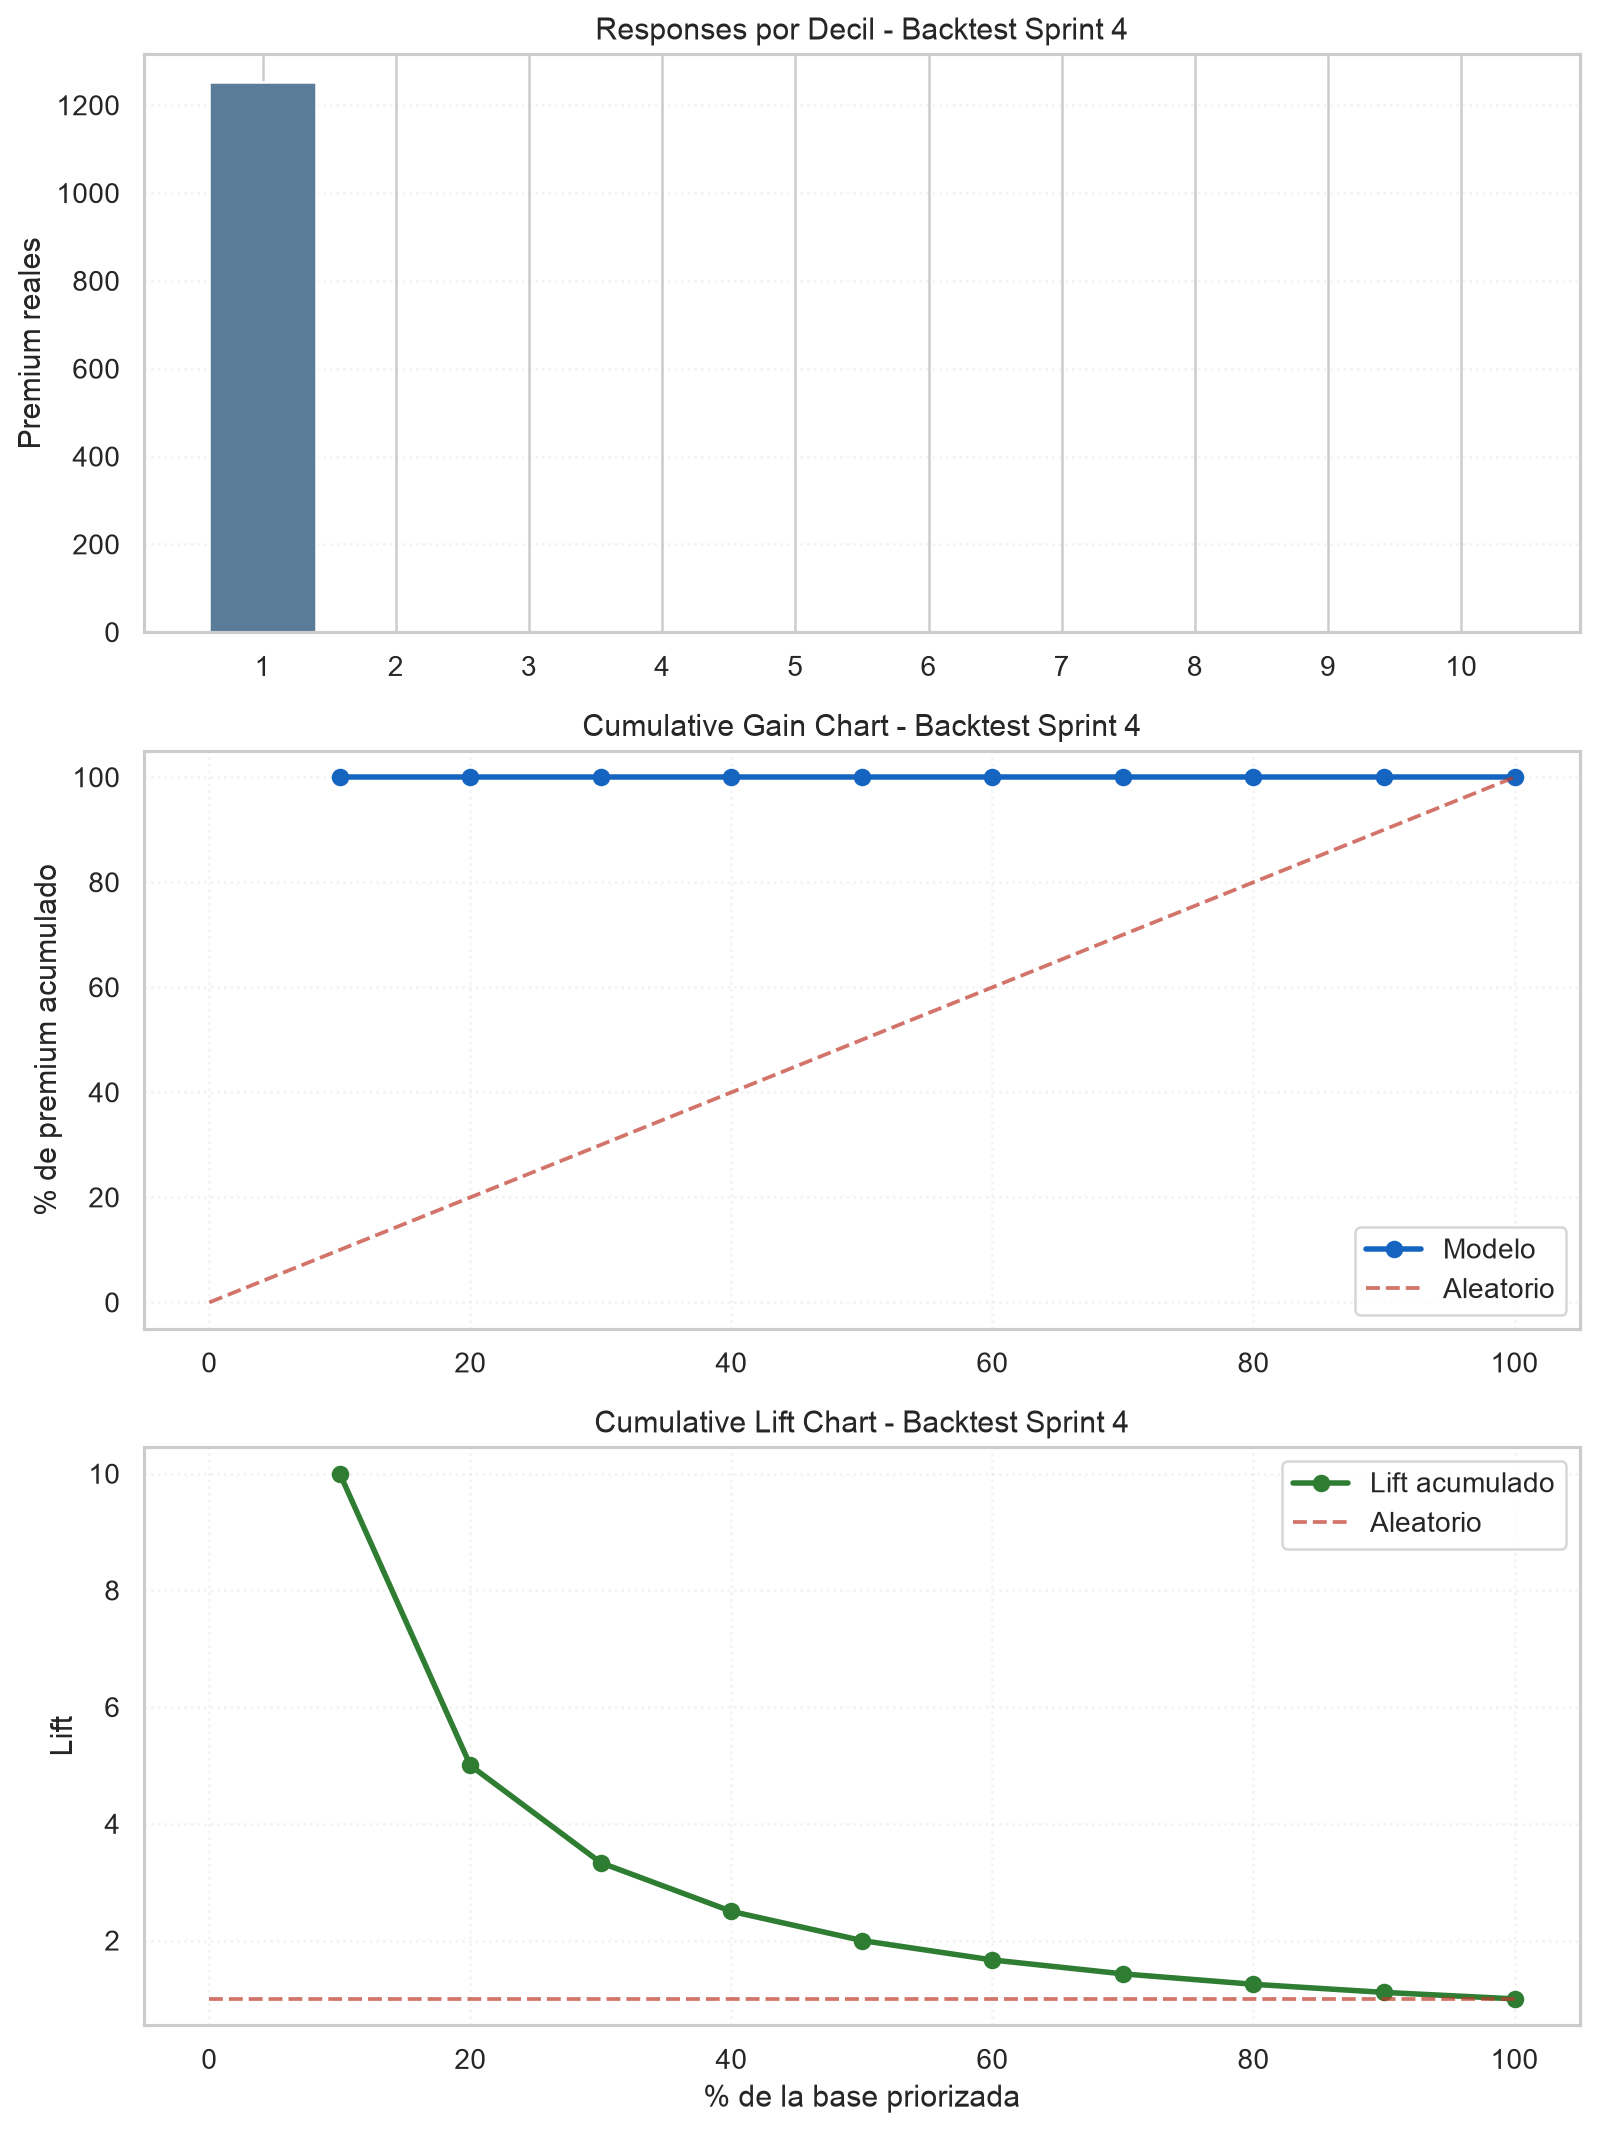
\includegraphics[width=\columnwidth]{sprint_04_backtest_gain_lift.png}
  \caption{Responses por decil y curvas acumuladas de gain/lift sobre el backtest oficial. Se observa que todos los premium reales del backtest quedan contenidos en el primer decil, aunque dicho decil no sea 100\% premium.}
  \label{fig:gain_lift_backtest}
\end{figure}

\begin{figure}[h]
  \centering
  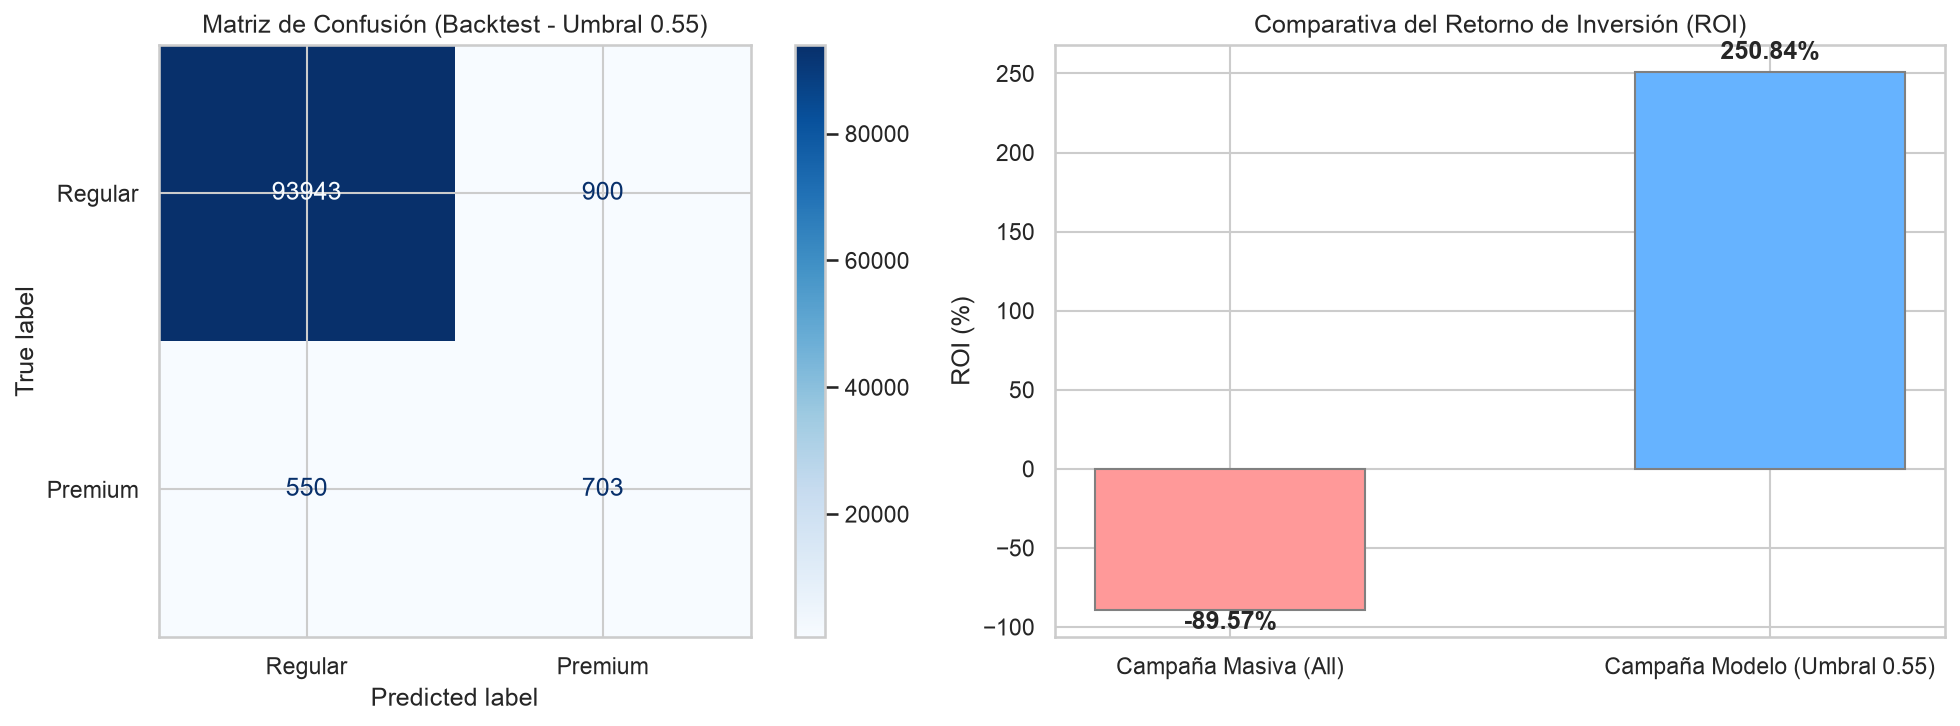
\includegraphics[width=\columnwidth]{sprint_04_holdout_evaluation_roi.png}
  \caption{Matriz de confusión sobre backtest y comparativa de ROI entre campaña masiva y campaña optimizada por modelo.}
  \label{fig:roi}
\end{figure}

\section{Monitoreo Operativo y Criterio de Reentrenamiento}
El MVP de Sprint 4 no debe interpretarse como un artefacto estático válido para cualquier momento futuro. Dado que el modelo fue entrenado sobre comportamiento histórico, su utilidad depende de que la relación entre señales transaccionales, contexto logístico y definición de cliente premium se mantenga razonablemente estable en el tiempo.

\subsection{Qué debe monitorearse}
En una operación posterior al Demo Day, el dashboard o una capa de monitoreo debería revisar al menos cuatro grupos de señales:
\begin{itemize}
    \item \textbf{Desempeño discriminativo:} métricas como ROC-AUC, Gini, Precision y Recall sobre ventanas nuevas no usadas en entrenamiento.
    \item \textbf{Impacto comercial:} ROI observado o estimado de la campaña focalizada frente a una estrategia masiva o baseline operativo.
    \item \textbf{Estabilidad poblacional:} tasa predicha de clientes premium y volumen de clientes efectivamente priorizados.
    \item \textbf{Drift de variables clave:} cambios relevantes en \texttt{delivered\_orders}, \texttt{total\_items}, \texttt{max\_payment\_installments}, \texttt{customer\_state} o \texttt{top\_category\_is\_high\_value}.
\end{itemize}

\subsection{Cuándo revisar o reentrenar}
La recomendación metodológica es \textbf{no reentrenar por calendario fijo}, sino por evidencia de deterioro sostenido. Como criterio operativo inicial para el MVP, puede proponerse:
\begin{itemize}
    \item \textbf{Alerta amarilla:} caída de Gini superior al 20\% respecto al baseline de referencia o descenso consistente de precision comercial.
    \item \textbf{Alerta roja:} Gini por debajo de un umbral mínimo acordado con negocio, acompañado por deterioro del ROI o por un cambio brusco en la tasa premium predicha.
    \item \textbf{Revisión obligatoria:} drift simultáneo en varias variables dominantes del modelo, aun si la métrica agregada todavía luce aceptable.
\end{itemize}

\subsection{Base temporal correcta para reentrenar}
Si se confirma degradación, el nuevo entrenamiento debe construirse sobre una \textbf{ventana temporal más reciente y completa}, separada del período usado por el artefacto vigente. Esta distinción es importante: mostrar resultados mes a mes sobre historia ya vista por el modelo puede servir como backtesting descriptivo del negocio, pero no como prueba suficiente de vigencia futura. En consecuencia, el reentrenamiento debe apoyarse en datos nuevos y comparables, no solo en recombinar la misma historia conocida.

\section{Gobernanza y Riesgos}
El Sprint 4 también consolidó una lectura de riesgo para uso responsable del MVP:
\begin{itemize}
    \item \textbf{Sesgo logístico/geográfico:} variables de tiempos de entrega y estimación pueden capturar desigualdades regionales.
    \item \textbf{Sesgo por bancarización:} señales como cuotas y método de pago pueden favorecer perfiles con mayor acceso financiero.
    \item \textbf{Necesidad de supervisión humana:} el score se propone como apoyo a priorización comercial, no como criterio automático único.
\end{itemize}

\section{Conclusiones}
El Sprint 4 logró cerrar el ciclo de integración entre analítica y producto:
\begin{enumerate}
    \item Se reutilizó el pipeline para construir un dataset de backtest alineado al artefacto oficial.
    \item Se implementó un MVP en Streamlit y una API mínima reproducibles en Docker.
    \item Se validó el modelo sobre backtest con métricas técnicas, explicabilidad y simulación de impacto.
    \item Se documentaron riesgos éticos, pitch ejecutivo y checklist final de cierre.
\end{enumerate}

La principal advertencia metodológica del sprint es que el backtest presenta un escenario más separable que la validación del Sprint 3. Por ello, el ROC-AUC de 0.9876 debe defenderse como resultado de un problema más fácil y de una etiqueta fuertemente ligada al comportamiento transaccional, no como una prueba aislada de superioridad definitiva del modelo.

\begin{thebibliography}{1}

\bibitem{sprint3_report}
M. de la Quintana, G. Nina, y G. Toro,
``Reporte de Sprint 3: Hiperparametrización, Selección del Modelo Final y Exportación del Clasificador de Clientes Premium,''
\textit{Informe Técnico, Módulo de Implementación de Soluciones de IA, Maestría en IA y Ciencia de Datos}, junio 2026.

\bibitem{lightgbm2017}
G. Ke, Q. Meng, T. Finley, T. Wang, W. Chen, W. Ma, Q. Ye, and T.-Y. Liu,
``LightGBM: A Highly Efficient Gradient Boosting Decision Tree,''
in \textit{Advances in Neural Information Processing Systems (NeurIPS)}, vol. 30, 2017.

\end{thebibliography}

\end{document}
